% TODO L07 REQUIREMENTS

\ifuniversity{tubs}{\date{December 2, 2025}}

\author{Thomas Thüm}
\lecture{Requirements}{requirements}

\begin{frame}{November 28, 2025: Airbus A320 Failure}
	\begin{fancycolumns}[widths={40}]
			\pic[width=\linewidth]{failures/airbus-a320}
			\begin{note}{}
				\begin{itemize}
					\item flight control software of 6,000 Airbus A320 affected
					\item quick fix: install old version of the software
				\end{itemize}
			\end{note}
		\nextcolumn
			\picDark[width=\linewidth]{failures/airbus-solar-radiation}
	\end{fancycolumns}
\end{frame}

\begin{frame}<3>{Recap: Reasons for Positive Test Cases} % copied from 03c-blackboxtesting
	\begin{fancycolumns}
		\begin{note}{Reasons for Positive Test Cases}
			\begin{itemize}
				\item actual fault
				\uncover<2->{\item wrong test case (input and expected results do not match)}
				\uncover<3->{\item interaction with other programs/libraries
					\item fault in the compiler
					\item fault in the operating system / device drivers
					\item fault in the hardware or hardware defect
					\item not enough memory
					\item does not halt (cf.\ undecidability of the halting problem)
					\item \emph{bitflip due to cosmic ray}
					\item \ldots}
			\end{itemize}
		\end{note}
	\end{fancycolumns}
\end{frame}

\begin{frame}{\insertsubtitle}
	\hprojectcartoon{01}{how the customer explained it}
	\hprojectcartoon{02}{how the project leader understood it}
	\alt<3->{%
		\projectcartoon{03}{how the analyst designed it}
		\projectcartoon{04}{how the programmer implemented it}
	}{%
		\hprojectcartoon{03}{how the analyst designed it}
		\hprojectcartoon{04}{how the programmer implemented it}
	}%
	\uncover<2->{\hprojectcartoon{13}{what the customer really needed}}
\end{frame}

\section{Introduction to Requirements}
\input{content/07a-requirements}
\lessonslearned{
	\item What kind of requirements exist and why?
	\item User and System Requirements Document \deutsch{Lasten- und Pflichtenheft}
	\item Next: Where do requirements come from?
}{
	\item \sommerville\mychapter{2.2.1}\mypages{54--55}
	\item \sommerville\mychapter{4.1}\mypages{101--111}
	\item \sommerville\mychapter{4.4.4}\mypages{126--128}
}{
	\begin{enumerate}
		\item Form groups of 2--3 students
		\item On your own: write down 1--2 own examples for a requirement
		\item Group work: classify each others requirements in groups of 2--3 students
		\item Try to find an example for each of the four categories: functional, non-functional (product, organizational, and external)
	\end{enumerate}
	Hint: Keep written requirements for a later interaction
}

\section{Elicitation of Requirements}
\subsection{Imprecise Requirements}
\begin{frame}{\insertsubsection}
	\begin{fancycolumns}[animation=none]
		\begin{note}{\sommerville:}
			\mycite{Imprecision in the requirements specification can lead to disputes between customers and software developers. It is natural for a system developer to interpret an ambiguous requirement in a way that simplifies its implementation. Often, however, this is not what the customer wants. New requirements have to be established and changes made to the system. Of course, this delays system delivery and increases costs.}
		\end{note}
		\nextcolumn
		\renewcommand{\projectcartoonwidth}{.3}
		\pause\hprojectcartoon{02}{how the project leader understood it}
		\hprojectcartoon{04}{how the programmer implemented it}
		\hprojectcartoon{13}{what the customer really needed}
	\end{fancycolumns}
\end{frame}

\subsection{Complete and Consistent Requirements}
\begin{frame}{\insertsubsection}
	\begin{fancycolumns}
		\begin{definition}{Completeness and Consistency \mysource{\sommerville}}
			\mycite{Ideally, the functional requirements specification of a system should be both complete and consistent. \emph{Completeness} means that all services and information required by the user should be defined. \emph{Consistency} means that requirements should not be contradictory.}
		\end{definition}	
		\begin{note}{Further Desired Properties}
			clear, easy to understand, unambiguous, correct, verifiable, prioritized, changeable, traceable %\deutsch{eindeutig, korrekt, überprüfbar, priorisiert, änderbar, nachvollziehbar}
		\end{note}
		\nextcolumn
		\begin{example}{Often not Feasible in Practice}
			mistakes, omission, implicit knowledge, many stakeholders \deutsch{Akteure} with different backgrounds / expectations / inconsistent needs
		\end{example}
	\end{fancycolumns}
\end{frame}

\begin{frame}[b]
	\begin{fancycolumns}
		\vspace{2mm}
		\pic[width=\linewidth,trim=0 175 0 75,clip]{people/fred-brooks}
		\vspace{-7mm}
		
		\begin{note}{Fred Brooks (1931--2022) \mysource{\href{https://ieeexplore.ieee.org/document/1663532}{Brooks 1987}}}
			\mycite{Much of the essence of building a program is in fact the debugging of the specification.}
		\end{note}
	\end{fancycolumns}
\end{frame}

\subsection{Requirements Engineering Process}
\begin{frame}{\insertsubsection} % TODO define term requirements engineering?
	\begin{fancycolumns}[columns=3,widths={80}]
		\begin{definition}{Requirements Elicitation and Analysis \mysource{adapted from \sommerville}}
			Requirements elicitation and analysis is the process of deriving the system requirements through observation of existing systems, discussions with potential users, or development of prototypes. \deutsch{Anforderungsermittlung und -analyse} 
		\end{definition}
		\nextcolumn
		\nextcolumn
	\end{fancycolumns}
	\begin{fancycolumns}[columns=3,widths={10,80,10}]
		\nextcolumn
		\begin{definition}{Requirements Specification \mysource{\sommerville}}
			\mycite{Requirements specification is the process of writing down the user and system requirements in a requirements document (aka. requirements specification).} \deutsch{Anforderungsspezifikation}
		\end{definition}
		%Requirements specification is the activity of translating the information gathered during requirements analysis into a document that defines a set of requirements (incl. user and system requirements).
		\nextcolumn
	\end{fancycolumns}
	\begin{fancycolumns}[columns=3,widths={10,10,80}]
		\nextcolumn
		\nextcolumn
		\begin{definition}{Requirements Validation \mysource{\sommerville}}
			\mycite{Requirements validation  is an activity that checks the requirements for realism, consistency, and completeness.} \deutsch{Anforderungsvalidierung}
		\end{definition}
	\end{fancycolumns}
\end{frame}
% TODO replace picture with tikz? simplify it? add in SE2 in more detail?
%\pause\pic[width=\linewidth]{sommerville/p55-f2.4}

\subsection{Why is Requirements Elicitation so Hard?}
\begin{frame}{\insertsubsection}
	\begin{fancycolumns}[animation=none,widths={66}]
		\begin{example}{}
			\begin{itemize}
				\item Stakeholders have difficulties to articulate what they want
				\item Stakeholders do not know what is (in)feasible
				\item Implicit knowledge and jargon in the customer's domain
				\item Dynamic business environment (e.g., new stakeholders)
			\end{itemize}
		\end{example}
	\end{fancycolumns}
\end{frame}

\subsection{Example Dialog by Ludewig and Lichter}
\begin{frame}{\insertsubsection}
	\begin{fancycolumns}[animation=none]
		\begin{itemize}
			\item At the morning you unlock the door at the main entrance?
			\item Every morning?
			\item Even at the weekend?
			\item And during the plant shutdown?
			\item And if you are sick or in holidays?
			\item And if Mr. X is off?
			\item What does \mycite{morning} mean?
		\end{itemize}
		\nextcolumn\vspace{5mm}
		\begin{itemize}
			\item Yes, as I said.
			\item Of course.
			\item No, at weekend the entrance remains closed.
			\item Clearly, it is then closed as well.
			\item Mr. X opens the door in this case.
			\item Then, a client knocks at the window to tell that the door is closed.
			\item \ldots
		\end{itemize}
	\end{fancycolumns}
	\vspace{5mm}
	
	Source: \ludewiglichter
	
	\href{https://youtu.be/NEUNEmJQGMw?t=1156}{Skit on Youtube (in German)}
\end{frame}

\subsection{Requirements Elicitation Techniques}
\begin{frame}{\insertsubsection}
	\begin{fancycolumns}[keep]
		\begin{definition}{Techniques for Requirement Elicitation}
			\begin{itemize}
				\item Open interviews: talk to users what they do
				\item Closed interviews: stakeholders answer predefined questions
				\item Ethnography: observation of stakeholder's work
				\item Prototyping
				\item Feedback loops
			\end{itemize}
		\end{definition}
		\nextcolumn
		\begin{note}{\sommerville:}
			\mycite{You need to spend time understanding how people work,
				what they produce, how they use other systems, and how they may need to change to accommodate a new system.}
		\end{note}
		\begin{example}{In Practice}
			Combinations of numerous techniques used
		\end{example}
	\end{fancycolumns}
\end{frame}

\subsection{Requirements Validation}
\begin{frame}{\insertsubsection}
	\begin{fancycolumns}[animation=none,widths={75}]
		\begin{note}{Motivation}
			The later problems with requirements are detected, the more costly it will be to fix them.
		\end{note}
		\begin{definition}{Requirements Validation}
			\setlength\tabcolsep{1mm}
			\begin{tabularx}{\textwidth}{rX}
				\emph{Validity checks} & do requirements (still) reflect real needs?\\
				\emph{Consistency checks} & are there contradictory/redundant requirements?\\
				\emph{Completeness checks} & are all functions and constrains documented?\\
				\emph{Realism checks} & is it feasible within budget and schedule?\\
				\emph{Verifiability} & can we test the requirements?
			\end{tabularx}
			
			~\\Checked by reviews, prototyping, and test-case creation
		\end{definition}
	\end{fancycolumns}
\end{frame}

\subsection{Recap: V-Model}
\begin{frame}{\insertsubsection} % slide copied from 06b-vmodel
	\begin{fancycolumns}
		\begin{definition}{V-Model \mysource{\ludewiglichter}}
			\begin{itemize}
				\item developed by the German Ministry of Defense \deutsch{Verteidigungsministerium} and required since 1992
				\item extension of the waterfall model: project-aligned activities such as quality assurance, configuration management, project management
				\item 1997 V-model 97: incremental development, inclusion of hardware, object-oriented development
				\item 2004 V-model XT (for extreme tailoring): adaptability, application beyond software
				% four project types of V-model XT
				\item integration of four testing stages
				%\item distinction between validation (right product) and verification (product correct)
				% fake? proposed 1979 by Barry Boehm
			\end{itemize}
		\end{definition}
		\nextcolumn
		\diagramVModel
		% TODO find reference for this kind of V model
	\end{fancycolumns}
\end{frame}


\lessonslearned{
	\item Desired properties for requirements
	\item Requirements engineering process?
	\item Techniques for requirements elicitation
	\item Next: How to document requirements graphically?
}{
	\item \sommerville\mychapter{4.2--4.3}\mypages{111--119}
	\item \sommerville\mychapter{4.5}\mypages{129f}
}{
	\begin{enumerate}% TODO animation of practical tasks does not work. remove animations everywhere?
		\item Form groups of 2--3 students
		\item On your own: reconsider your written examples and write down improved versions
		\item Group work: let your colleagues guess what property you aimed to improve
	\end{enumerate}
	Hint: Recap on desired properties: complete, consistent, clear, easy to understand, unambiguous, correct, verifiable, prioritized, changeable, traceable
}

\section{Documentation of Requirements}
\subsection{Natural Language Specification}
\begin{frame}{\insertsubsection}
	\begin{fancycolumns}[widths={55}]
		\begin{definition}{}
			\begin{itemize}
				\item used since 1950s
				\item since programmer is not necessarily the user
			\end{itemize}
		\end{definition}
		\begin{example}{Style Guidelines}
			\begin{itemize}
				\item one or two short sentences of natural language
				\item one message per sentence
				\item use active voice (e.g., \mycite{the system \ldots})
				\item consistent use of language (i.e., avoid synonyms)
				\item use shall for mandatory and should for desirable requirements
				\item use text highlighting
				\item avoid jargon, abbreviations, acronyms
				\item provide a rationale
			\end{itemize}
		\end{example}
		\nextcolumn
		\begin{note}{Pros}
			\begin{itemize}
				\item expressive
				\item intuitive
				\item universal
			\end{itemize}
		\end{note}
		\begin{note}{Cons}
			\begin{itemize}
				\item vague \deutsch{vage}
				\item ambiguous \deutsch{mehrdeutig}
				\item interpretation depends on reader's background
			\end{itemize}
		\end{note}
	\end{fancycolumns}
\end{frame}

\subsection{Structured Specifications}
\begin{frame}{\insertsubsection}
	\begin{fancycolumns}[widths={55}]
		\begin{definition}{}
			\begin{itemize}
				\item use of templates rather than free-form text
				\item distinguishes between function, description, input (origin), output (destination), pre- and postconditions, side effects, rationale, dependencies to other requirements, \ldots
				\item or any subset thereof
				\item user stories are typically structured specifications
			\end{itemize}
		\end{definition}
		\begin{example}{Example}
			\setlength\tabcolsep{1mm}
			\begin{tabularx}{\textwidth}{rX}
				Function & Exchange of IDs\\
				Description & Two devices send their IDs to each other.\\
				Precondition & Devices have been within a distance of 2m for at least 15 minutes.\\
				Postcondition & IDs are stored in the local database.\\
				Rationale & Contact tracing requires to temporarily identify the device of contacts.
			\end{tabularx}
		\end{example}
		\nextcolumn
		\begin{note}{Pros}
			\begin{itemize}
				\item {\color{gray} expressive}
				\item {\color{gray} intuitive}
				\item information easier to find
				\item less likely to forget certain information (e.g., rationale)
			\end{itemize}
		\end{note}
		\begin{note}{Cons}
			\begin{itemize}
				\item {\color{gray} vague}
				\item {\color{gray} ambiguous}
				\item {\color{gray} interpretation depends on reader's background}
				\item same structure can be too restrictive
				\item multiple structures can be confusing
			\end{itemize}
		\end{note}
	\end{fancycolumns}
\end{frame}

\subsection{Use Case Diagrams}
\begin{frame}[label=usecaseslide]{\insertsubsection\ \normalsize(since 1993)}
	\begin{fancycolumns}[animation=none]
		\begin{definition}{Use Case Diagram \deutsch{Anwendungsfalldiagramm}}
			Use case diagrams are a means to capture the requirements of systems, i.e., what systems are supposed to do. The key concepts specified in this diagram are actors, use cases, and subjects:%\\~
			\begin{itemize}
				\item Each \emph{subject} represents a system under consideration to which the use case applies. \deutsch{System}
				\item Each users and any other system that may interact with a subject is represented as an \emph{actor}. \deutsch{Akteur}
				\item A \emph{use case} is a specification of behavior in terms of verb and noun. \deutsch{Anwendungsfall}
			\end{itemize}
			\mysource{adapted from \umlspec}
		\end{definition}
		\nextcolumn
		%\posthandout{\pic[width=\linewidth,trim=0 50 25 40,clip]{blackboard/blackboard_use_case1_23_24}}
		%\posthandout{\pic[page=44,width=\linewidth,trim={.5\width} {.1\height} {.02\width} {.2\height},clip]{se09-requirements-print}}
		\posthandout{\pic[page=50,width=\linewidth,trim=225 20 15 40,clip]{printedslides/2021wt/requirements}}
	\end{fancycolumns}
\end{frame}

\begin{frame}{Example}
	\posthandout{\centering\pic[page=51,width=.9\linewidth,trim=25 20 25 0,clip]{printedslides/2021wt/requirements}}
\end{frame}

\subsection{Include and Extend Relationships}
\begin{frame}[label=includeandextendslide]{\insertsubsection}
	\begin{fancycolumns}[animation=none]
		\begin{definition}{Include Relationship}
			\textbf{Motivation}: make common parts of multiple use cases explicit%\\[1mm]
			
			\textbf{Relationship}: a \emph{base use case} may define an include relationship to an \emph{included use case}%\\[1mm]
			
			\textbf{Meaning}: included use case is always executed when the base use case is
		\end{definition}
		\begin{definition}{Extend Relationship}
			\textbf{Motivation}: make explicit that some use cases only happen under certain circumstances%\\[1mm]
			
			\textbf{Relationship}: an \emph{extend use case} may define an extend relationship to a \emph{base use case}%\\[1mm]
			
			\textbf{Meaning}: when the base use case is executed, the extend use case may or may not be executed
		\end{definition}
		\nextcolumn
		\posthandout{\pic[page=53,width=\linewidth,trim=225 20 15 50,clip]{printedslides/2021wt/requirements}}
		%\posthandout{\pic[page=46,width=\linewidth,trim={.5\width} {.2\height} {.02\width} {.2\height},clip]{se09-requirements-print}}
	\end{fancycolumns}
\end{frame}

% TODO add rules for use case diagrams

% TODO discuss advantages/disadvantages of use case diagrams

% TODO combination of textual and visual requirements

\pictureframe{
	\pic[width=\paperwidth]{emotions/walking-on-water}
}{
	\vspace{65mm}
	\begin{note}{Edward V. Berard (1993) \mysource{\href{https://en.wikiquote.org/wiki/Edward_V._Berard}{wikiquote.org}}}
		\mycite{Walking on water and developing software from a specification are easy if both are frozen.}
	\end{note}
}

\lessonslearned{
	\item Natural language and structured specification of requirements
	\item Graphical specification with use case diagrams \deutsch{Anwendungsfalldiagramme}
	\item Next: How to model the system behavior in more detail?
}{
	\item \sommerville\mychapter{4.4}\mypages{120--126}
	\item \sommerville\mychapter{5.2.1}\mypages{144--146}
	\item \umlspec\mychapter{18}
}{
	Quiz in Stud.IP
	\lectureqr{07}
}

%\faq{
	%	\item
	%}{
	%	\item
	%}{
	%	\item
	%}

\input{template/footer}

% TODO L08 SYSTEM MODELING

\ifuniversity{tubs}{\date{December 9, 2025}}

\author{Thomas Thüm}
\lecture{System Modeling}{modeling}

% TODO blackboard on graphical notation: use case vs system vs activity vs state

\begin{frame}{\insertsubtitle}
	\hprojectcartoon{01}{how the customer explained it}
	\hprojectcartoon{02}{how the project leader understood it}
	\alt<3->{%
		\projectcartoon{03}{how the analyst designed it}
		\projectcartoon{04}{how the programmer implemented it}
	}{%
		\hprojectcartoon{03}{how the analyst designed it}
		\hprojectcartoon{04}{how the programmer implemented it}
	}%
	\uncover<2->{\hprojectcartoon{13}{what the customer really needed}}
\end{frame}

\section{Introduction to Modeling}
\subsection{Motivation for Modeling}
\begin{frame}{\insertsubsection}
	\begin{fancycolumns}
		\begin{note}{\umluserguide:}
			\mycite{A successful software organization is one that consistently deploys \emph{quality software} that meets the needs of its users. An organization that can develop such software in a \emph{timely and predictable} fashion, with an \emph{efficient and effective use of resources}, both human and material, is one that has a sustainable business.
				
				[...]
				
				Modeling is a central part of all the activities that lead up to the deployment of good software. We build models to \emph{communicate} the desired structure and behavior of our system. We build models to \emph{visualize and control} the system's architecture. We build models to better \emph{understand} the system we are building, often exposing opportunities for \emph{simplification and reuse}. And we build models to \emph{manage risk}.}
		\end{note}
		\nextcolumn
		\begin{note}{\umluserguide:}
			\mycite{We build models of complex systems because we cannot comprehend such a system in its entirety.}
		\end{note}
	\end{fancycolumns}
\end{frame}

\begin{frame}[b]{Recap: Software Engineering vs Programming}
	\slideSEvsProgramming
\end{frame}

\begin{frame}
	\begin{fancycolumns}
		\pic[width=\linewidth,trim=0 300 0 80,clip]{people/bjarne-stroustrup}
		\vspace{-7mm}
		
		\begin{note}{Bjarne Stroustrup (2000) \mysource{\cpp}}
			\mycite{The most important single aspect of software development is to be clear about what you are trying to build.}
		\end{note}
	\end{fancycolumns}
\end{frame}

\subsection{What is System Modeling?}
\begin{frame}{\insertsubsection}
	\begin{fancycolumns}
		\begin{definition}{System Modeling \mysource{\sommerville}}
			\mycite{\emph{System modeling} is the process of developing abstract models of a system, with each model presenting a different view or perspective of that system. [...] Models are used during the requirements engineering process to help derive the \emph{detailed requirements} for a system, during the design process to \emph{describe the system to engineers} implementing the system, and after implementation to \emph{document the system}’s structure and operation.}
		\end{definition}
	\end{fancycolumns}
\end{frame}

\subsection{What is a Model?}
\begin{frame}{\insertsubsection}
	\begin{fancycolumns}
		\begin{definition}{\umluserguide:}
			\mycite{A \emph{model} is a simplification of reality.}
		\end{definition}
		\begin{definition}{\sommerville:}
			\mycite{A \emph{model} is an abstract view of a system that deliberately ignores some system details.}
		\end{definition}
		\begin{note}{{Goals of Models \mysource{\umluserguide}}}
			\begin{itemize}
				\item visualize a system as it is (wanted)
				\item specify the structure or behavior of a system
				\item template to guide construction of a system
				\item document the decisions we have made
			\end{itemize}
		\end{note}
		\nextcolumn
		\begin{note}{\sommerville:}
			\mycite{It is important to understand that a system model is \emph{not a complete representation} of system. It purposely leaves out detail to make it \emph{easier to understand}. A model is an abstraction of the system being studied rather than an alternative representation of that system. A representation of a system should maintain all the information about the entity being represented. An abstraction \emph{deliberately simplifies a system} design and picks out the most salient characteristics.}
		\end{note}
	\end{fancycolumns}
\end{frame}

\subsection{What Language to Use for Modeling?}
\begin{frame}{\insertsubsection}
	\begin{fancycolumns}
		\myexample{Towards a Common Language}{
			\begin{itemize}
				\item Natural language? hard to abstract from details, already used in requirements
				\item Programming language? unfamiliar to people without programming skills in that language, too early to decide for the programming language
				\item Textual language? harder to understand
				\item Graphical language? makes use of our visual abilities, requires common understanding
				\item Problem: engineers need to be aware of all languages being used
				\item Solution: use a graphical language independent of company and domain
			\end{itemize}
		}
	\end{fancycolumns}
\end{frame}

% TODO new slides on History of Modeling Languages?

\xkcdframe{927} % 14+1 standards

\subsection{The Unified Modeling Language (UML)}
\begin{frame}{\insertsubsection}
	\begin{fancycolumns}
		\begin{definition}{UML \mysource{\umlrefman}}
			\mycite{The Unified Modeling Language (UML) is a general-purpose visual modeling language that is used to specify, visualize, construct, and document the artifacts of a software system.}
		\end{definition}
		\pause
		\begin{note}{\umluserguide:}
			\mycite{Modeling yields an understanding of a system. No one model is ever sufficient. Rather, you often need multiple models that are connected to one another [...].}
		\end{note}
	\end{fancycolumns}
\end{frame}

\subsection{Different Kinds of UML Diagrams}
\begin{frame}{\insertsubsection}
	\begin{fancycolumns}
		\begin{definition}{Structure Diagrams \deutsch{Strukturdiagramme}}
			\mycite{\emph{Structure diagrams} show the static structure of the objects in a system. That is, they depict those elements in a specification that are irrespective of time. The elements in a structure diagram represent the meaningful concepts of an application, and may include abstract, real-world and implementation concepts.}\mysource{\umlspec}
		\end{definition}	
		\nextcolumn
		\begin{definition}{Behavior Diagrams \deutsch{Verhaltensdiagramme}}
			\mycite{\emph{Behavior diagrams} show the dynamic behavior of the objects in a system, including their methods, collaborations, activities, and state histories. The dynamic behavior of a system can be described as a series of changes to the system over time.}\mysource{\umlspec}
		\end{definition}
	\end{fancycolumns}
\end{frame}
% TODO add paragraph on interaction diagrams?

\subsection{14 Types of UML Diagrams}
\begin{frame}{\insertsubsection\ \mytitlesource{\umlspec}}
	\only<-4>{\tikzset{notTaughtUMLDiagrams/.style={}}}%
	\only<-5|handout:0>{\slideMindmapUMLdiagrams{}{}{}{}{}{}{visible on={<2->}}{visible on=<3->}{visible on=<4->}}%
	\only<6|handout:0>{\slideMindmapUMLdiagrams{blue}{}{}{}{}{}{}{}{}}%
	\only<7->{\slideMindmapUMLdiagrams{blue}{red}{red}{}{}{}{}{}{}}%
	
	\uncover<5->{Six most important UML diagrams* discussed in this course
		
		*\tiny\href{https://dl.acm.org/doi/10.1145/1278201.1278205}{John Erickson and Keng Siau. 2007. Theoretical and practical complexity of modeling methods. Commun. ACM 50, 8 (August 2007), 46–51.}}
\end{frame}

% TODO talk about SysML? or at least mention in the slides?

\lessonslearned{
	\item System modeling
	\item Models as abstractions
	\item UML and its visual languages
	\item Next: How to model activities of a system?
}{
	\item[] \umluserguide\mychapter{1} --- great introduction to modeling
}{
	\begin{enumerate}
		\item Form groups of 2--3 students
		\item In isolation: Practice abstraction by sketching this lecture hall in \href{https://webuhr.de/timer-auf-1-minute/}{1 minute} (not more!).
		\item Groupwork: Show the sketch to your group and discuss what details are not shown in your visualizations. (5 min)
	\end{enumerate}
}

\section{Modeling Behavior with Activity Diagrams}
\xkcdframe{844}

\subsection{Activity Diagrams}
\begin{frame}{\insertsubsection}
	\begin{fancycolumns}[animation=none]
		\posthandout{\picWhite[page=18,width=\linewidth,trim=15 20 225 40,clip]{printedslides/2021wt/modeling}}
		%\posthandout{\pic[page=3,width=\linewidth,trim=60 140 450 150,clip]{modeling/09-modeling_drawings}}
		\nextcolumn
		\begin{definition}{Activity Diagram \deutsch{Aktivitätsdiagramm}}
			An \emph{activity diagram} is a diagram visualizing activities and their order of execution. An activity diagram contains \emph{activities} (rounded box) that are connected by means of \emph{flows} (solid arrows). The execution begins at the \emph{initialization} (filled circle) and ends with the \emph{completion} node (bull's eye). \deutsch{Aktivität, Fluss, Startzustand, Endzustand}
		\end{definition}
		\pause%
		\begin{note}{Rules for Activity Diagrams}
			\begin{itemize}
				\item exactly one initialization node
				\item at least one activity
				\item every activity has one incoming and one outgoing flow
				\item every activity is reachable from initialization
				\item completion is reachable from every activity
			\end{itemize}
		\end{note}
		% What is the difference between activity and action? \umluserguide
	\end{fancycolumns}
\end{frame}

% TODO make sure that example contains activities (i.e., not only nouns)
\begin{frame}{Example of Sequential Activities}
	\posthandout{\picWhite[page=19,width=\linewidth,trim=0 20 0 40,clip]{printedslides/2021wt/modeling}}
%	\posthandout{\pic[page=4,width=\linewidth,trim=60 80 80 120,clip]{modeling/09-modeling_drawings}}
\end{frame}

\subsection{Branching and Merging in Activity Diagrams}
\begin{frame}{\insertsubsection}
	\begin{fancycolumns}[animation=none]
		\posthandout{\picWhite[page=20,width=\linewidth,trim=25 20 225 40,clip]{printedslides/2021wt/modeling}}
		%\posthandout{\pic[page=5,width=\linewidth,trim=60 120 450 150,clip]{modeling/09-modeling_drawings}}
		\nextcolumn
		\begin{definition}{{Branching and Merging \mysource{\umluserguide}}}
			\textbf{Motivation}: model control flow that depends on certain conditions (i.e., actions that may happen)
			
			\textbf{Branching}: A \emph{branch} has exactly one incoming and two or more outgoing flows. Each outgoing flow has a Boolean expression called \emph{guard}, which is evaluated on entering the branch. \deutsch{Verzweigung}
			
			\textbf{Merging}: A \emph{merge} has two or more incoming and exactly one outgoing flow. \deutsch{Zusammenführung}
		\end{definition}
		\pause
		\begin{note}{Further Rules for Activity Diagrams}
			\begin{itemize}
				\item guards on outgoing flows should not overlap (flow of control is unambiguous)
				\item guards should cover all possibilities (flow of control does not freeze)
				\item keyword \emph{else} possible for one guard \deutsch{sonst}
			\end{itemize}
		\end{note}
	\end{fancycolumns}
\end{frame}

\begin{frame}{Example of Conditional Activities}
	\posthandout{\picWhite[page=21,width=\linewidth,trim=0 20 0 40,clip]{printedslides/2021wt/modeling}}
	%\posthandout{\pic[page=1,width=\linewidth,trim=60 80 80 150,clip]{modeling/09-modeling_drawings}}
\end{frame}

\subsection{Forking and Joining in Activity Diagrams}
\begin{frame}{\insertsubsection}
	\begin{fancycolumns}[animation=none]
		\posthandout{\picWhite[page=22,width=\linewidth,trim=25 20 225 40,clip]{printedslides/2021wt/modeling}}
		%\posthandout{\pic[page=2,width=\linewidth,trim=60 140 450 120,clip]{modeling/09-modeling_drawings}}
		\nextcolumn
		\begin{definition}{{Forking and Joining \mysource{\umluserguide}}}
			\textbf{Motivation}: model concurrent control flows (i.e., activities that run in parallel)
			
			\textbf{Forking}: A \emph{fork} (thick horizontal or vertical line) has exactly one incoming and two or more outgoing flows. \deutsch{Gabelung}
			
			\textbf{Joining}: A \emph{join} (thick horizontal or vertical line) has two or more incoming and exactly one outgoing flow. \deutsch{Vereinigung}
		\end{definition}
		\pause
		\begin{note}{Further Rules for Activity Diagrams}
			\begin{itemize}
				\item branched paths must be merged eventually \deutsch{letztendlich}
				\item forked paths must be joined eventually
				\item only outgoing edges of branch nodes have guards
			\end{itemize}
		\end{note}
	\end{fancycolumns}
\end{frame}

	\begin{frame}{Example of Concurrent Activities}
		\posthandout{\picWhite[page=23,width=\linewidth,trim=0 20 0 40,clip]{printedslides/2021wt/modeling}}
		%\posthandout{\pic[page=6,width=\linewidth,trim=60 100 10 120,clip]{modeling/09-modeling_drawings}}
	\end{frame}

\subsection{Swimlanes in Activity Diagrams}
\begin{frame}{\insertsubsection}
	\begin{fancycolumns}[animation=none]
		\posthandout{\picWhite[page=24,width=\linewidth,trim=20 20 225 40,clip]{printedslides/2021wt/modeling}}
		%\posthandout{\pic[page=1,width=\linewidth,trim=60 100 150 150,clip]{modeling/09-modeling_drawings}}
		\nextcolumn
		\begin{definition}{{Swimlanes \mysource{\umluserguide}}}
			\textbf{Motivation}: group activities according to responsibilities
			
			\textbf{Swimlane}: An activity diagram may have no or at least two swimlanes. A \emph{swimlane} (rectangle) represents a high-level responsibility activities within an activity diagram. \deutsch{Verantwortlichkeitsbereiche}
		\end{definition}
		\pause
		\begin{note}{Further Rules for Activity Diagrams}
			\begin{itemize}
				\item each swimlane has a name unique within its diagram
				\item every activity belongs to exactly one swimlane
				\item only flows may cross swimlanes
			\end{itemize}
		\end{note}
	\end{fancycolumns}
\end{frame}

\begin{frame}{Recap: 14 Types of UML Diagrams\ \mytitlesource{\umlspec}}
	\slideMindmapUMLdiagrams{blue}{blue}{red}{}{}{}{}{}{}
\end{frame}


\lessonslearned{
	\item UML activity diagrams
	\item Branching and merging
	\item Forking and joining
	\item Swimlanes
	\item Next: How to model states of a system?
}{
	\item[] \umluserguide\mychapter{20}
	% less suited introduction: \sommerville, Chapter 5.1 (p.\ 141--144)
}{
	\begin{enumerate}
		\item Form groups of 2--3 students
		\item Draw a activity diagram for an instant messenger by yourself.
		\item It should contain at least one branch or fork. You are free to use swimlanes.
		\item Exchange your diagrams within your group and look for mistakes.
	\end{enumerate}
}

\section{Modeling Behavior with State Machines}
\input{content/08c-statemachines}
\lessonslearned{
	\item UML state machine diagrams
	\item Hierarchical state machines
	\item Next: How to structure a system into subsystems?
}{
	\item[] \umluserguide\mychapter{22} 
	% less suited introduction: \sommerville, Chapter 5.4.2 (p.\ 156--158)
}{
	Quiz in Stud.IP
	\lectureqr{08}
}

%\faq{
	%	\item
	%}{
	%	\item
	%}{
	%	\item
	%}

\input{template/footer}

% TODO L09 SOFTWARE ARCHITECTURE

\ifuniversity{tubs}{\date{December 16, 2025}}

\author{Thomas Thüm}
\lecture{Software Architecture}{architecture}

\begin{frame}{\insertsubtitle}
	\alt<2->{%
		\projectcartoon{01}{how the customer explained it}
		\projectcartoon{02}{how the project leader understood it}
	}{%
		\hprojectcartoon{01}{how the customer explained it}
		\hprojectcartoon{02}{how the project leader understood it}
	}%
	\hprojectcartoon{03}{how the analyst designed it}
	\alt<2->{%
		\projectcartoon{04}{how the programmer implemented it}
		\projectcartoon{13}{what the customer really needed}
	}{%
		\hprojectcartoon{04}{how the programmer implemented it}
		\hprojectcartoon{13}{what the customer really needed}
	}%
\end{frame}

\section{Introduction to Software Architecture}
\subsection{On the Role of Architecture}
\begin{frame}{\insertsubsection}
	\begin{fancycolumns}
		\centering
		\pic[height=60mm]{misc/ulm-muenster} % TODO remove and replace by other building?
	\end{fancycolumns}
\end{frame}

\begin{frame}{Architecture Bridges the Gap}
	\begin{fancycolumns}[columns=3,animation=none]
		\uncover<4->{
			\begin{example}{}
				Large software systems \ldots
				\begin{itemize}
					\item have numerous requirements
					\item require many developers
					\item need separation of concerns\\\deutsch{Trennung von Belangen}
				\end{itemize}
			\end{example}
		}
		\nextcolumn
		\nextcolumn
		\uncover<3->{
			\begin{note}{}
				\mycite{Weeks of coding can save you hours of planning.}\mysource{anon}
			\end{note}
		}
	\end{fancycolumns}
	\begin{tikzpicture}[xscale=4.95]
		\node[label=below:Requirements] (req) at (0,0) {\pic[height=2.5cm]{architecture/requirements}};
		\only<2->{\node[label=below:Implementation] (code) at (2,0) {\pic[height=2.5cm]{architecture/source-code}};}
		%\only<2>{\node[label=below:Softwarearchitektur] (swa) at (.95,0) {\includegraphics[height=1.9cm]{component-diagram}};}
		\only<5->{
			\draw[->,line width=5pt,gray] (req) -- (code);
			\node[label=below:Software Architecture] (swa) at (.95,0) {\pic[height=2.5cm]{architecture/component-diagram-large}};
		}
	\end{tikzpicture}
\end{frame}

\subsection{Recap: Process Models}
\begin{frame}[10]{\insertsubsection}
	\begin{fancycolumns}[widths={45}]
		\diagramWaterfallModel
		\nextcolumn
		\diagramVModel
	\end{fancycolumns}
\end{frame}

\subsection{Software Architecture}
\begin{frame}{\insertsubsection\ \mytitlesource{\sommerville}}
	\begin{fancycolumns}[keep]
		\begin{definition}{Architectural Design \deutsch{Architekturentwurf}}
			\mycite{\emph{Architectural design} is a creative process in which you design a system organization that will satisfy the functional and non-functional requirements of a system.}
		\end{definition}
		\pause
		\begin{definition}{Software Architecture}
			\mycite{A \emph{software architecture} is a description of how a software system is organized. Properties of a system such as performance, security, and availability are influenced by the architecture used.}
		\end{definition}
		\nextcolumn
		\pause
		\begin{example}{In Practice:}
			\mycite{You might propose an abstract system architecture where you associate groups of system functions or features with large-scale components or subsystems. You then use this decomposition to discuss the requirements and more detailed features of the system with stakeholders.}
		\end{example}
	\end{fancycolumns}
\end{frame}

\xkcdframe{2347}

\subsection{3 Goals of Software Architecture}
\begin{frame}{\insertsubsection\ \normalsize[\sommerville]}
	\begin{fancycolumns}[columns=1] % hack to make mindmap visible in dark mode
		\centering{\tikz[grow cyclic,
			mindmap, every node/.style=concept,concept color=red!20!background,
			%text width=20mm,align=flush center,
			level 1/.append style={level distance=27mm,sibling angle=360/3}]
			\node {Goals of Software Architectures}
			[clockwise from=210]
			child[visible on=<2->] { node {meet critical requirements} }
			child[visible on=<3->] { node {communication of stakeholders} }
			child[visible on=<4->] { node {support software reuse} }
			;}
	\end{fancycolumns}
\end{frame}

\subsection{4 Views in Software Architecture}
\begin{frame}{\insertsubsection\ \normalsize[\sommerville]}
	\begin{fancycolumns}[keep]
		{\tikz[grow cyclic,
			mindmap, every node/.style=concept,concept color=blue!20!background,
			%text width=20mm,align=flush center,
			level 1/.append style={level distance=27mm,sibling angle=360/4}]
			\node {Architectural Views}
			[clockwise from=225]
			child[visible on=<2->] { node {logical view} }
			child[visible on=<3->] { node {process view} }
			child[visible on=<4->] { node {development view} }
			child[visible on=<5->] { node {physical view} }
			;}
		\nextcolumn
		\begin{definition}{\sommerville:}
			\small
			\mycite{\uncover<2->{A \emph{logical view}, which shows the key abstractions in the system as objects or object classes. It should be possible to relate the system requirements to entities in this logical view.}
				
				\uncover<3->{A \emph{process view}, which shows how, at runtime, the system is composed of interacting processes. This view is useful for making judgments about non-functional system characteristics such as performance and availability.}
				
				\uncover<4->{A \emph{development view}, which shows how the software is decomposed for development; that is, it shows the breakdown of the software into components that are implemented by a single developer or development team. This view is useful for software managers and programmers.}
				
				\uncover<5->{A \emph{physical view}, which shows the system hardware and how software components are distributed across the processors in the system. This view is useful for systems engineers planning a system deployment.}}
		\end{definition}
	\end{fancycolumns}
\end{frame}

\subsection{Conway's Law}
\begin{frame}
	\begin{fancycolumns}[height=8.5cm]
		\pic[width=\linewidth,trim=0 50 0 0,clip]{people/melvin-conway}
		\vspace{-7mm}
		
		\begin{note}{Melvin E. Conway (1968) \mysource{\href{http://www.melconway.com/Home/Committees_Paper.html}{melconway.com}}}
			Conway's Law: \mycite{Any organization that designs a system [...] will produce a design whose structure is a copy of the organization's communication structure.}
		\end{note}
	\end{fancycolumns}
\end{frame}

\lessonslearned{
	\item Software architecture: decomposition into subsystems
	\item Goals: communication, reuse, critical requirements
	\item Views: physical, logical, process, development
	\item Next: How to model the components of a system?
}{
	\item[] \sommerville\mychapter{6.0--6.2}\mypages{167--175}
}{
	\begin{enumerate}
		\item[] Invest five minutes trying to understand the Signal messenger by inspecting the \href{https://github.com/signalapp/Signal-Android}{source code of the Android client}
		%\item Answer questionnaire
	\end{enumerate}
	\lectureqr{09}
}
%\only<3->{
%  \item[A] Ich habe ein gutes Verständnis wie die App funktioniert.
%  \item[B] Ich habe ein grobes Verständnis wie die App aufgebaut ist.
%  \item[C] Ich habe einen kleinen Teil der App verstanden.
%  \item[D] Ich habe genug verstanden, um morgen an der App zu entwickeln.
%  \item[E] Ich habe nichts wesentliches verstanden und möchte die 5 Minuten Lebenszeit zurück.
%}

\section{Modeling Structure with Component Diagrams}
\begin{frame}{Recap: 14 Types of UML Diagrams\ \mytitlesource{\umlspec}}
	\slideMindmapUMLdiagrams{blue}{blue}{blue}{red}{}{}{visible on={<2->}}{}{}
\end{frame}

\subsection{Component Diagrams}
\begin{frame}[label=componentslide]{\insertsubsection\ \deutsch{Komponentendiagramm}}
	\begin{fancycolumns}[animation=none]
		\begin{definition}{Component Diagram \mysource{adapted from \umluserguide}}
			A \emph{component} is a replaceable part of a system that conforms to and provides the realization of a set of interfaces. An \emph{interface} is a collection of operations that specify a service that is provided by or requested from a class or component. An interface that a component realizes is called a \emph{provided interface}, meaning an interface that the component provides as a service to other components. The interface that a component uses is called a \emph{required interface}, meaning an interface that the component conforms to when requesting services from other components. \deutsch{Komponente, angebotene/benötigte Schnittstelle}
		\end{definition}
		\nextcolumn
		\posthandout{\picWhite[page=16,width=\linewidth,trim=225 20 25 40,clip]{printedslides/2021wt/architecture}}
	\end{fancycolumns}
\end{frame}

\begin{frame}{Example of a Component Diagram}
	\posthandout{\picWhite[page=17,width=\linewidth,trim=0 20 0 40,clip]{printedslides/2021wt/architecture}}
\end{frame}

% TODO all current examples are missing situations in which a provided interface is to more than 1 required interfaces

\subsection{Hierarchical Component Diagrams}
\begin{frame}[label=nestedcomponentsslide]{\insertsubsection}
	\begin{fancycolumns}[animation=none]
		\begin{definition}{Nesting of Components\mysource{adapted from \umluserguide}}
			\textbf{Motivation}: decompose/structure large systems
			
			\textbf{Nesting} \deutsch{Verschachtelung}: A component may contain any number of \emph{subcomponents}. \deutsch{Teilkomponenten}
			
			\textbf{Ports and Delegates}: A \emph{port} is an explicit window into an encapsulated component. A \emph{delegate} connects provided or required interfaces with ports. 
		\end{definition}
		\nextcolumn
		\posthandout{\picWhite[page=18,width=\linewidth,trim=225 20 25 40,clip]{printedslides/2021wt/architecture}}
	\end{fancycolumns}
\end{frame}

\subsection{Rules for Component Diagrams}
\begin{frame}{\insertsubsection}
	\begin{fancycolumns}
		\begin{note}{Rules for Component Diagrams}
			\begin{itemize}
				\item component names are unique
				\item a component may have any number of required or provided interfaces
				\item every required interface is connected to provided interface
				\item every component is directly or indirectly connected to every other component
				\item subcomponents may be nested to any level
				\item when subcomponents communicate to a higher-level component, they need to communicate via ports
			\end{itemize}
		\end{note}
	\end{fancycolumns}
\end{frame}

\begin{frame}
	\begin{fancycolumns}[height=8.5cm]
		\pic[width=\linewidth,trim=175 0 0 0,clip]{people/gordon-bell}
		\vspace{-7mm}
		
		\begin{note}{Gordon Bell \mysource{\href{https://dl.acm.org/doi/10.1145/1968.381154}{Bentley 1984}}}
			\mycite{The cheapest, fastest, and most reliable components are those that aren’t there.}
		\end{note}
	\end{fancycolumns}
\end{frame}

\begin{frame}{Recap: 14 Types of UML Diagrams\ \mytitlesource{\umlspec}}
	\only<1|handout:0>{\slideMindmapUMLdiagrams{blue}{blue}{blue}{blue}{}{}{}{}{}}%
	\only<2->{\slideMindmapUMLdiagrams{blue}{blue}{blue}{blue}{red}{red}{}{}{}}%
\end{frame}

\lessonslearned{
	\item UML component diagrams
	\item Decompose of large systems with nesting
	\item Next: What architectures have been successful?
}{
	\item[] \umluserguide\mychapter{15} 
	% less suited: \sommerville, Chapter 5.4.2 (p.\ 156--158)
}{
	\begin{enumerate}
		\item Form groups of 2--3 students
		\item Design the architecture of a messenger with a component diagram with \emph{exactly one} mistake.
		\item Exchange diagrams with each other, and try to identify and mark the mistake.
	\end{enumerate}
}

\section{Common Architectural Patterns}
\input{content/09c-architecturalpatterns}
\lessonslearned{
	\item[] Common architectural patterns: layered architecture, client-server, 3-tier, peer-to-peer, model-view-controller, pipe-and-filter
	\item Next: How to model behavior within components?
}{
	\item \sommerville\mychapter{6.3}\mypages{175--184}
}{
	Quiz in Stud.IP
	\lectureqr{09}
}

%\faq{
	%	\item
	%}{
	%	\item
	%}{
	%	\item
	%}

\input{template/footer}

% TODO L10 SOFTWARE DESIGN

\ifuniversity{tubs}{\date{January 6, 2026}}

\author{Thomas Thüm}
\lecture{Software Design}{design}

\begin{frame}{\insertsubtitle}
	\alt<2->{%
		\projectcartoon{01}{how the customer explained it}
		\projectcartoon{02}{how the project leader understood it}
	}{%
		\hprojectcartoon{01}{how the customer explained it}
		\hprojectcartoon{02}{how the project leader understood it}
	}%
	\hprojectcartoon{03}{how the analyst designed it}
	\hprojectcartoon{04}{how the programmer implemented it}
	\alt<2->{%
		\projectcartoon{13}{what the customer really needed}
	}{%
		\hprojectcartoon{13}{what the customer really needed}
	}%
\end{frame}

\begin{frame}{Tired of Swings? What about Bikes?}
	\xkcd{1673}{width=\linewidth}
\end{frame}

\section{Modeling Interactions with Sequence Diagrams}
\input{content/10a-sequencediagrams}
\lessonslearned{
	\item Software design
	\item Connection to requirements and architecture
	\item UML sequence diagrams
	\item Notation and semantics of roles, lifelines, (stacked) activity, (a)synchronous message, return
	\item Next: How to model structure within components?
}{
	\item[] \sommerville\mychapter{7.0--7.1} % TODO identify which of the pages are relevant to this part 196--209
	\item \umlrefman\mychapter{9}
	\item \umluserguide\mychapter{19}
}{
	Quiz in Stud.IP % identify syntactically wrong sequence diagrams
	\lectureqr{10}
}

\section{Modeling Structure with Class Diagrams}
\begin{frame}{Recap: 14 Types of UML Diagrams\ \mytitlesource{\umlspec}}
	\centering\slideMindmapUMLdiagrams{blue}{blue}{blue}{blue}{red}{}{}{visible on={<-0>}}{}
\end{frame}

\subsection{Class Diagrams}
\begin{frame}{\insertsubsection\ \normalsize\deutsch{Klassendiagramme}}
	\begin{fancycolumns}[animation=none]
		\begin{definition}{{Class Diagram\mysource{\umluserguide}}}
			%\mycite{A \emph{class diagram} shows a set of classes, interfaces, and collaborations and their relationships.}
			\mycite{A \emph{class} is a description of a set of objects that share the same attributes, operations, relationships, and semantics. [...] 
				\uncover<2->{ An \emph{association} is a structural relationship that specifies that objects of one thing are connected to objects of another. [...]}
				\uncover<3->{When a class participates in an association, it has a specific role that it plays in that relationship; a \emph{role} is just the face the class at the far end of the association presents to the class at the near end of the association. [...]}
				\uncover<4->{When you state a \emph{multiplicity} at the far end of an association, you are specifying that, for each object of the class at the near end, how many objects at the [far] end may exist.}}
		\end{definition}
		\uncover<5->{\small
			\begin{example}{{Example Multiplicities (default=*)}\mysource{\umlrefman}}
				0..* (=*) or 1..* or 0..1 or 1..1 (=1) \ldots\ 2..5 \ldots
			\end{example}
			% default is actually unspecified, meaning that it take any value which is close to *
			% source: \umlrefman and https://coderanch.com/t/100225/engineering/defualt-multiplicity
		}
		\nextcolumn
		\posthandout{\picWhite[page=13,width=\linewidth,trim=225 20 20 40,clip]{printedslides/2021wt/design}}
		%\mynote{\umluserguide:}{\mycite{Class diagrams are the most common diagram found in modeling object-oriented systems.}}
		% deliberatively ignore: fully qualified names such as java::awt::Rectangle, active classes, packages, dependencies, association names
	\end{fancycolumns}
\end{frame}

\subsection{Attributes and Operations of Classes}
\begin{frame}{\insertsubsection}
	\begin{fancycolumns}[widths={51},animation=none]
		\begin{definition}{{Attributes and Operations \mysource{\umluserguide}}}
			\mycite{An \emph{attribute} is a named property of a class that describes a range of values that instances of the property may hold. [...]%
				\uncover<2->{ An \emph{operation} is the implementation of a service that can be requested from any object of the class to affect behavior. In other words, an operation is an abstraction of something you can do to an object that is shared by all objects of that class.}} 
			\uncover<3->{\emph{Static} attributes and operations exist only once for each class and are underlined (opposed to \emph{instance} ones).}
		\end{definition} % \deutsch{Attribute und Operationen)
		\uncover<4->{
			\begin{definition}{{Visibility Modifiers \mysource{\umluserguide}}}
				\begin{itemize}
					\item[\emph{--}] private is available only in this class
					\item[\emph{+}] public is available from each class
					\item[\emph{\#}] protected is available from each subclass
					\item[\emph{\raisebox{-0.9ex}{\~{}}}] package is available in classes of same package
				\end{itemize}
			\end{definition}
		}
		% TODO add primitive types? Int, Float, Boolean
		% deliberatively ignore: responsibilities, modeling of own primitive types
		\nextcolumn
		\posthandout{\picWhite[page=14,width=\linewidth,trim=225 20 20 40,clip]{printedslides/2021wt/design}}
	\end{fancycolumns}
\end{frame}
	
\subsection{Completeness of Attributes and Operations}
\begin{frame}{\insertsubsection}
	\begin{fancycolumns}
		\begin{note}{\umluserguide:}
			\mycite{When drawing a class, you don't have to show every attribute and every operation at once. In fact, in most cases, you can't (there are too many of them to put in one figure) and you probably shouldn't (only a subset of these attributes and operations are likely to be relevant to a specific view). For these reasons, you can elide a class, meaning that you can choose to show only some or none of a class's attributes and operations.}
		\end{note}
	\end{fancycolumns}
\end{frame}

\subsection{Aggregation and Composition of Classes}
\begin{frame}{\insertsubsection}
	\begin{fancycolumns}[animation=none]
		\begin{definition}{{Aggregation \mysource{adapted from \umluserguide}}}
			\emph{Aggregation} is a special association in which one class represents a larger thing (the whole), which consists of smaller things (the parts) (i.e., has-a relationship). In contrast, a plain association between two classes represents a structural relationship between peers, meaning that both classes are conceptually at the same level.
		\end{definition}
		\uncover<2->{
			\begin{definition}{{Composition \mysource{\umluserguide}}}
				\mycite{\emph{Composition} is a form of aggregation, with strong ownership and coincident lifetime as part of the whole. Parts with non-fixed multiplicity may be created after the composite itself, but once created they live and die with it. Such parts can also be explicitly removed before the death of the composite.}
			\end{definition}
		}
		\nextcolumn
		\posthandout{\picWhite[page=16,width=\linewidth,trim=225 20 20 40,clip]{printedslides/2021wt/design}}
	\end{fancycolumns}
\end{frame}

\widexkcdframe{2309}

\subsection{Inheritance Relationships}
\begin{frame}{\insertsubsection}
	\begin{fancycolumns}[animation=none]
		\begin{definition}{Generalization and Abstract Classes}
			\mycite{A \emph{generalization} is a relationship between a general kind of thing (called the superclass or parent) and a more specific kind of thing (called the subclass or child). Generalization is sometimes called an is-a-kind-of relationship: one thing is-a-kind-of a more general thing.} If a superclass cannot be instantiated it is an \emph{abstract class} (also denoted with \textit{italic name}). \deutsch{Generali-\\sierung, abstrakte Klasse}\mysource{\umluserguide}
		\end{definition}
		\uncover<2->{
			\begin{definition}{Interfaces and Realization}
				An \emph{interface} is a special class that only has static non-private attributes, abstract non-private operations, cannot be instantiated, and not be in a generalization relationship. Classes may \emph{realize} an interface. \deutsch{Schnittstelle, Realisierung}
			\end{definition}
		}
		\nextcolumn
		\posthandout{\picWhite[page=18,width=\linewidth,trim=225 20 20 40,clip]{printedslides/2021wt/design}}
	\end{fancycolumns}
\end{frame}

\subsection{Rules and Hints for Class Diagrams}
\begin{frame}{\insertsubsection}
	\begin{fancycolumns}
		\begin{note}{Rules for Class Diagrams}
			\begin{itemize}
				\item Class and attribute names are short nouns or noun phrases
				\item Operation names are verbs or short phrases starting with verbs
				\item Use camel case, whereas the first letter of attributes and operations is not capitalized
				\item A class has an arbitrary number of attributes/operations, any subset thereof shown in a diagram
				\item No cycles in inheritance relationships
				\item Abstract operations only live in abstract classes
				\item Interfaces cannot have private members (attributes/operations)
				\item Each class can only be a \textbf{part} of one composition
			\end{itemize}
		\end{note}
		\nextcolumn
		\begin{example}{{Hints on Inheritance \mysource{\umluserguide}}}
			\mycite{An object of the child class may be used for a variable or parameter typed by the parent, but not the reverse. In other words, generalization means that the child is substitutable for a declaration of the parent. A child inherits the properties of its parents, especially their attributes and operations. Often—but not always—the child has attributes and operations in addition to those found in its parents. An implementation of an operation in a child overrides an implementation of the same operation of the parent; this is known as polymorphism. To be the same, two operations must have the same signature (same name and parameters).}
		\end{example}
	\end{fancycolumns}
\end{frame}

\begin{frame}{Recap: 14 Types of UML Diagrams\ \mytitlesource{\umlspec}}
	\centering\slideMindmapUMLdiagrams{blue}{blue}{blue}{blue}{blue}{blue}{}{}{}%
	
	\uncover<2->{Six most important UML diagrams* discussed in this course
		
		*\tiny\href{https://dl.acm.org/doi/10.1145/1278201.1278205}{John Erickson and Keng Siau. 2007. Theoretical and practical complexity of modeling methods. Commun. ACM 50, 8 (August 2007), 46–51.}}
\end{frame}

\lessonslearned{
	\item UML class diagrams
	\item Notation and semantics of association, role, multiplicity, (static) attribute, (static/abstract) operation, visibility modifiers, aggregation, composition, generalization, abstract class, interface, realization
	\item Next: How can we discuss software designs without diagrams?
}{
	\item[] \umluserguide\mychapter{4, 5, 9, 10} 
}{
	\begin{enumerate}
		\item<+-> Form groups of 2--3 students
		\item In isolation: Sketch a class diagram with 3--5 classes for a software of your choice. However, add exactly three errors violating the rules of class diagrams. \deutsch{Fehlersuchbild}
		\item Group work: Exchange your diagrams with each other. Find and mark the errors with another color.
	\end{enumerate}
}

\section{Common Design Patterns}
\subsection{Design Patterns}
\slideDesignPatterns

\subsection{Gang of Four}
\slideGangOfFour

\subsection{Creational Design Patterns}
\begin{frame}{\insertsubsection{} \mytitlesource{\gof}}
	\centering\slideMindmapDesignPatterns{}{notTaughtDesignPatterns}{notTaughtDesignPatterns}{}{notTaughtDesignPatterns}{}{visible on={<-0|handout:0>}}{}{visible on={<-0|handout:0>}}
\end{frame}

\subsection{Singleton Pattern}
\begin{frame}{\insertsubsection}
	\begin{fancycolumns}
		\begin{definition}{Singleton \mysource{\gofen}}
			\setlength\tabcolsep{1mm}
			\begin{tabularx}{\textwidth}{rX}				
				intent & \mycite{Ensure a class [has only] one instance, and provide a global point of access to it.}\\
				% aka. & \\
				motivation & avoid the uncontrolled creation of multiple instances\\
				idea & a private constructor is called on class initialization and a public static method is used for access to that single instance
			\end{tabularx}
		\end{definition}
		\nextcolumn
		\centering\only<2|handout:0>{\singleton{width=.1\linewidth}}
		\only<3->{\singleton{width=.5\linewidth}}
	\end{fancycolumns}
\end{frame}

\begin{frame}{\insertsubsection: Example}
	\begin{fancycolumns}
		\begin{definitiontight}{Pattern}
			\centering\singleton{width=.5\linewidth}		
		\end{definitiontight}
		\nextcolumn
		\begin{exampletight}{Example Application}
			\centering\singletonexample{width=.5\linewidth}
		\end{exampletight}
	\end{fancycolumns}
\end{frame}

\begin{frame}[t]{\insertsubsection{} \mytitlesource{\umlrefman\mypages{91--92,198--199,387--388}; \umluserguide\mypages{318--323}; \umlspec\mypages{217--218}}}
	\alt<2->{\profcalculatorcollaboration{width=\linewidth,page=4}}{\profcalculatorcollaboration{width=\linewidth,page=6}}
	
	\vspace{-70mm}
	\begin{fancycolumns}[widths={70},animation=none]
		\nextcolumn
		\mynotetight{Singleton Pattern}{\singleton{width=\linewidth}}
	\end{fancycolumns}
\end{frame}

\subsection{Structural Design Patterns}
\begin{frame}{\insertsubsection{} \mytitlesource{\gof}}
	\centering\slideMindmapDesignPatterns{}{notTaughtDesignPatterns}{notTaughtDesignPatterns}{}{notTaughtDesignPatterns}{}{visible on={<2->}}{}{visible on={<-0|handout:0>}}
\end{frame}

\subsection{Object Adapter Pattern}
\begin{frame}{\insertsubsection}
	\begin{fancycolumns}
		\begin{definition}{Object Adapter \mysource{\gofen}}
			\setlength\tabcolsep{1mm}
			\begin{tabularx}{\textwidth}{rX}				
				intent & \mycite{Convert the interface of a class into another interface clients expect. Adapter lets classes work together that couldn't otherwise because of incompatible interfaces.}\\
				aka. & wrapper\\
				motivation & enable reuse of classes even though incompatible interfaces cannot be made compatible\\
				idea & create a new class with a compatible interface that forwards all requests
			\end{tabularx}
		\end{definition}
		\nextcolumn
		\objectadapter{width=\linewidth}
	\end{fancycolumns}
\end{frame}

\begin{frame}[t]{\insertsubsection{} \mytitlesource{\umlrefman\mypages{91--92,198--199,387--388}; \umluserguide\mypages{318--323}; \umlspec\mypages{217--218}}}
	\alt<2->{\profcalculatorcollaboration{width=\linewidth,page=2}}{\profcalculatorcollaboration{width=\linewidth,page=6}}
	
	\vspace{-75mm}
	\begin{fancycolumns}[widths={65},animation=none]
		\nextcolumn
		\mynotetight{Object Adapter Pattern}{\objectadapter{width=\linewidth}}
	\end{fancycolumns}
\end{frame}

\subsection{Behavioral Design Patterns}
\begin{frame}{\insertsubsection{} \mytitlesource{\gof}}
	\centering\slideMindmapDesignPatterns{}{notTaughtDesignPatterns}{notTaughtDesignPatterns}{}{notTaughtDesignPatterns}{}{}{}{visible on={<2->}}
\end{frame}

\subsection{Observer Pattern}
\begin{frame}{\insertsubsection}
	\begin{fancycolumns}
		\begin{definition}{Observer \mysource{\gofen}}
			\setlength\tabcolsep{1mm}
			\begin{tabularx}{\textwidth}{rX}				
				intent & \mycite{Define a one-to-many dependency between objects so that when one object changes state, all its dependents are notified and updated automatically.}\\
				aka. & dependents, publish-subscribe\\
				motivation & avoid coupling of classes (i.e., explicit references such as imports)\\
				example & no coupling between model and view in model-view-controller architectures\\
				idea & data object (model) has a list of observers (views) that are notified about changes
			\end{tabularx}
		\end{definition}
		\nextcolumn
		\observer{width=\linewidth}
	\end{fancycolumns}
\end{frame}

%\subsection{Overview on Design Patterns}
%\begin{frame}{\insertsubsection{} \mytitlesource{\gof}}
%	\only<-4|handout:0>{\tikzset{notTaughtDesignPatterns/.style={}}}%
%	\slideMindmapDesignPatterns{}{notTaughtDesignPatterns}{notTaughtDesignPatterns}{}{notTaughtDesignPatterns}{}{visible on={<1,4,5->}}{visible on={<2,4->}}{visible on={<3->}}
%\end{frame}


\lessonslearned{
	\item Design patterns are solution ideas to reoccuring design problems
	\item Creational patterns: Singleton
	\item Structural patterns: Object adapter
	\item Behavioral patterns: Observer
	\item Next: How to avoid implementing the same requirements again?
}{
	\item \gof\mychapter{3--5}
}{
	Questions?
%	Later: Quiz in Stud.IP
%	\lectureqr{11}
}

%\faq{
	%	\item
	%}{
	%	\item
	%}{
	%	\item
	%}

\input{template/footer}

% TODO L11 SOFTWARE REUSE

\ifuniversity{tubs}{\date{January 13, 2026}}

\author{Thomas Thüm}
\lecture{Software Reuse}{reuse}

\begin{frame}{\insertsubtitle}
	\alt<3->{%
		\projectcartoon{01}{how the customer explained it}
		\projectcartoon{02}{how the project leader understood it}
		\projectcartoon{03}{how the analyst designed it}
		\projectcartoon{04}{how the programmer implemented it}
	}{%
		\hprojectcartoon{01}{how the customer explained it}
		\hprojectcartoon{02}{how the project leader understood it}
		\hprojectcartoon{03}{how the analyst designed it}
		\hprojectcartoon{04}{how the programmer implemented it}
	}%
	\uncover<2->{\hprojectcartoon{16}{the open source version}}
\end{frame}

\section{Techniques for Reuse}
\subsection{Development of Similar Products: Elevators}
\begin{frame}{\insertsubsection}
	\uncover<5->{\begin{note}{}
		\centering All these elevators are different but also share similarities.
	\end{note}}

	~

	\begin{fancycolumns}[columns=4,T]
		\centering\pic[width=\linewidth]{elevators/elevator1-out}
		
		two buttons
	\nextcolumn
		\centering\pic[width=\linewidth]{elevators/elevator2-out2}
		
		one button
	\nextcolumn
		\centering\pic[width=\linewidth]{elevators/elevator3-out}
		
		keyhole
	\nextcolumn
		\centering\pic[width=\linewidth]{elevators/elevator2-out1}
		
		floor display
	\end{fancycolumns}
\end{frame}

\begin{frame}{\insertsubsection}
	\uncover<5->{\begin{note}{}
			\centering Shall we implement each product from scratch or can we reuse parts thereof?
	\end{note}}

	~

	\begin{fancycolumns}[columns=4,widths={28,21,28,21},T]
		\centering\pic[width=\linewidth]{elevators/elevator1-in2}
		
		no button to close door
	\nextcolumn
		\centering\pic[width=\linewidth]{elevators/elevator3-in1}
		
		two keyholes
	\nextcolumn
		\centering\pic[width=\linewidth]{elevators/elevator4-in}
		
		keycard
	\nextcolumn
		\centering\pic[width=\linewidth]{elevators/elevator2-in2}
		
		double tap for~undo
	\end{fancycolumns}
\end{frame}

\subsection{Reuse with Components}
\begin{frame}{\insertsubsection}
	\begin{fancycolumns}[animation=none]
		\picWhite[page=25,width=\linewidth,trim={.5\width} {.1\height} {.05\width} {.2\height},clip]{printedslides/2021wt/architecture}
	\nextcolumn
		\begin{definition}{Reuse with Client-Server Architectures}
			Different client components can communicate with the same server component
		\end{definition}
		\uncover<2->{\begin{note}{Discussion}
			\begin{itemize}
				\item Reuse of server component for multiple clients
				\item Lower effort than developing multiple servers
				\item Unit testing: only one server needs to be tested
				\item Integration testing: any change to the server may break an existing client
				\item Changing a client may require changes to the server or its interface (API); changing the server may require changes to all clients
				\item Challenge: how to design stable APIs?
			\end{itemize}
		\end{note}}
	\end{fancycolumns}
\end{frame}

\begin{frame}{\insertsubsection}
	\begin{fancycolumns}[animation=none]
		\picWhite[page=24,width=\linewidth,trim={.5\width} {.1\height} {.05\width} {.2\height},clip]{printedslides/2021wt/architecture}
		\nextcolumn
		\begin{definition}{Reuse with Layered Architectures}
			Layer can be replaced by compatible one with same interface (e.g., IP v4 by IP v6)
		\end{definition}
		\uncover<2->{\begin{note}{Discussion}
			\begin{itemize}
				\item Replacing some layers and reusing others
				\item Ideally only new layers need to be implemented
				\item In practice: adaptations to existing layers may be necessary
				\item Again: interplay needs to be checked with integration testing
				\item Challenge: how to design interoperable layers?
			\end{itemize}
		\end{note}}
	\end{fancycolumns}
\end{frame}

% TODO add log4j exploit here illustrating how often it was reused and how often it was vulnerable

\subsection{Reuse with Runtime Parameters}
\begin{frame}{\insertsubsection}
	\uncover<3->{\begin{definition}{}
		\centering All functionality implemented in one product. Parameters used to activate varying behavior.
	\end{definition}}
	\begin{fancycolumns}
		\pic[width=\linewidth]{reuse/runtime-parameters-win10-cmd-dir2}
	\nextcolumn
		\pic[width=\linewidth]{reuse/runtime-parameters-win10-cmd-dir}
	\end{fancycolumns}
\end{frame}

\begin{frame}{\insertsubsection}
	\begin{fancycolumns}[animation=none]
		\picDark[width=\linewidth,trim={.35\width} {.12\height} {.1\width} {.45\height},clip]{reuse/runtime-parameters} % \mysource{\featureide}
	\nextcolumn
		\begin{definition}{Reuse with Runtime Parameters}
			Complete product is reused and extended with new behavior (e.g., features on demand in cars)
		\end{definition}
		\uncover<2->{\begin{note}{Discussion}
				\begin{itemize}
					\item Configuration: reuse with new combination of existing parameters
					\item Extension: implementation of new parameters and parameter values
					\item Challenges:
						\begin{itemize}
							\item larger binaries compared to excluded components
							\item safety and security risks by unused functionality
							\item side effects: any change to a parameter may break other parameters
						\end{itemize}
				\end{itemize}
		\end{note}}
	\end{fancycolumns}
\end{frame}

\subsection{Ad-Hoc Reuse with Clone-and-Own}
\begin{frame}{\insertsubsection}
	\centering\trunkbranch{}{}
	\begin{fancycolumns}[T,widths={30}]
		\begin{definition}{Clone-and-Own}
			Complete product is copied (cloned) and modified as needed (owned)
			
			aka. cloning in the large
		\end{definition}
	\nextcolumn
		\begin{note}{Discussion}
				\begin{itemize}
					\item Copying often done by branching or forking in version control
					\item Fast and flexible implementation strategy for adaptation
					\item Challenges:
					\begin{itemize}
						\item features and adaptations lost in the implementation
						\item consistent changes of clones hardly possible in practice
						\item clones are an obstacle during evolution and maintenance
						\item no actual reuse, often considered an anti pattern
					\end{itemize}
				\end{itemize}
		\end{note}
	\end{fancycolumns}
\end{frame}

\lessonslearned{
	\item Development of similar products
	\item Reuse with components
	\item Reuse with runtime parameters
	\item Ad-hoc reuse with clone-and-own
	\item Next: When are we allowed to reuse software?
}{
	\item \sommerville\mychapter{15}\mychapter{16} 
}{
	Link to teaching evaluation in Stud.IP
	
	(group names without letters, e.g., 5A/5B as 5)
	\lectureqr{11}
}

\section{Open-Source Software}
\input{content/11b-opensource}
\lessonslearned{
	\item Open-source development and open-source software
	\item Examples and central questions around open source
	\item Copyleft and its impact on software
	\item Software licenses: MIT, GPL, LGPL
	\item Recommendations for companies
	\item Next: What did you learn in this course?
}{
	\item \sommerville\mychapter{7.4} Open-Source Development
}{
	\begin{enumerate}
		\item Form groups of 2--3 students
		\item Find three example for software systems were you would recommend any of the following licenses: MIT, GPL, LGPL
		\item What are reasons for the license over the other two licenses?
	\end{enumerate}
}

\section{Lecture Summary}
\subsection*{Topics of Software Engineering 1}
\begin{frame}{\myframetitle{}}
	\lectureseriesoverview[1]
\end{frame}
\begin{frame}{\myframetitle{}}
	\lectureseriesexplanation{}
\end{frame}

\subsection{Software Projects}
\subsubsection{Lecture 1+11: Software and Reuse}
\begin{frame}{Lecture 1: Software (Engineering) vs Program(ming)}
	\slideSEvsProgramming
\end{frame}
\begin{frame}{Lecture 11: How to avoid software development?}
	\begin{fancycolumns}[animation=none]
		\begin{note}{First Question}
			\mycite{Should the product that is being developed make use of open-source components?}
		\end{note}
		\begin{note}{Second Question}
			\mycite{Should an open-source approach be used for its own software development?}
		\end{note}
		\pic[width=.25\linewidth]{opensource/copyleft}\hfill\pic[width=.25\linewidth]{opensource/copyright}
	\nextcolumn
		\begin{exampletight}{}
			\centering\pic[width=.55\linewidth]{opensource/mit-logo}
		\end{exampletight}
		\begin{exampletight}{}
			\centering\pic[width=.55\linewidth]{opensource/gplv3-logo}
		\end{exampletight}
		\begin{exampletight}{}
			\centering\pic[width=.55\linewidth]{opensource/lgplv3-logo}
		\end{exampletight}
	\end{fancycolumns}
\end{frame}

\subsubsection{Lecture 5+6: Management}
\begin{frame}[2]{Lecture 5: How to manage software development?}
	\slideGanttAndNetwork
\end{frame}
\begin{frame}[10]{Lecture 6: How to structure software development?}
	\centering\diagramVModel
\end{frame}

\subsection{Analysis and Design}
\subsubsection{Lecture 7+8: Analysis}
\begin{frame}[1]{Lecture 7: What software is required?}
	\slideMindmapNonFunctionalRequirements
\end{frame}
\begin{frame}{Lecture 8: How to model the planned software?}
	\centering\slideMindmapUMLdiagrams{}{}{}{}{}{}{}{}{}
\end{frame}

\subsubsection{Lecture 9+10: Design}
\begin{frame}{Lecture 9: What is the high-level structure?}
	\begin{fancycolumns}[animation=none]
		\picWhite[page=16,width=\linewidth,trim=225 20 25 40,clip]{printedslides/2021wt/architecture}
	\nextcolumn
		\picWhite[page=26,width=\linewidth,trim=225 20 25 40,clip]{printedslides/2021wt/architecture}
	\end{fancycolumns}
\end{frame}
\begin{frame}{Lecture 10: What is the low-level structure?}
	\begin{fancycolumns}[animation=none]
		\picWhite[page=13,width=\linewidth,trim=225 20 20 40,clip]{printedslides/2021wt/design}
	\nextcolumn
		\objectadapter{width=\linewidth}
	\end{fancycolumns}
\end{frame}

\subsection{Implementation, Test, and Maintenance}

\subsubsection{Lecture 2: Implementation}
\begin{frame}[2]{Lecture 2: How to implement the software?}
	%\slideProgrammingLanguagesToday
	\picDark[width=\linewidth]{history/tiobe}
\end{frame}
\subsubsection{Lecture 3: Testing}
\begin{frame}{Lecture 3: How to test the software?}
	\slideMindmapQualityAssurance{}{}{}{}{}{}{}
\end{frame}

\subsubsection{Lecture 4: Maintenance}
\begin{frame}[2]{Lecture 4: How to maintain the software?}
	\slideEvolutionAndMaintenance
\end{frame}
%\begin{frame}{Lecture 5: How to control changes?}
%	\centering\picDark[width=.75\linewidth]{versioncontrol/devops}
%\end{frame}

%\begin{frame}{Software Engineering I}
%	\vspace{-5mm}
%	\renewcommand{\projectcartoonwidth}{.13}
%	\small\hfill
%	\hprojectcartoon{01}{requirements}
%	\hprojectcartoon{02}{modeling}
%	\hprojectcartoon{03}{architecture and design} % architecture/design
%	\hprojectcartoon{04}{implementation}\\\hfill
%	\hprojectcartoon{05}{testing} % testing
%	\hprojectcartoon{06}{process}
%	%\hprojectcartoon{07}{how the project was documented} % code documentation
%	%\hprojectcartoon{08}{what operations installed} % devops/continuous integration
%	\hprojectcartoon{09}{management and pricing} % pricing
%	%\hprojectcartoon{10}{how it was supported}
%	%\hprojectcartoon{11}{what marketing advertised}
%	%\hprojectcartoon{12}{when it was delivered} % continous delivery
%	\uncover<2->{\hprojectcartoon{13}{Software Engineering II}}
%	%\hprojectcartoon{14}{what the digg effect can do to your site} % ???
%	%\hprojectcartoon{15}{the disaster recover plan}
%	%\hprojectcartoon{16}{how open source version} % open source/licensing
%	%\hprojectcartoon{17}{how it performed under load} % quality assurance/performance
%	%\hprojectcartoon{18}{how patches were applied} % software maintenance
%	
%\end{frame}

\lessonslearned{
	\item How to avoid / manage / structure software development?
	\item What software is required?
	\item How to model / design / implement / test / change / maintain software?
	\item Next: SEP Topic Presentation (next week)
}{
	\item[] See previous lectures
}{
	Questions?
}
	%	\small
	%	\item[1.] Software, its impacts, its engineering
	%	\item[2.] Requirements, different kinds, its engineering, use case diagrams
	%	\item[3.] System modeling, UML, activity/state machine diagrams
	%	\item[4.] Software architecture, component diagrams, architectural patterns
	%	\item[5.] Software design, class/sequence diagrams
	%	\item[6.] Implementation, programming languages, coding conventions, tooling
	%	\item[7.] Design patterns, structural (object adapter, composite, decorator), creational (singleton, abstract factory), behavioral (observer)
	%	\item[8.] Quality assurance, compilation, code reviews, white-box/black-box testing
	%	\item[9.] Process models, Waterfall, V-Model, Scrum
	%	\item[10.] Project management, planning, scheduling

%\faq{
	%	\item
	%}{
	%	\item
	%}{
	%	\item
	%}

\input{template/footer}
